\section{Этапы проектирования конструкции РЭС и их характеристика}

Во время работы в малом предприятии трудно заметить
четкие границы перехода между этапами конструирования РЭС,
так как процесс конструирования, кроме того, что увлекателен сам по себе,
в данном случае ещё и не усложнён бюрократической волокитой,
а также нуждой согласовывать каждый этап.
Хотя это можно также списать на тот факт,
что во время прохождения практики я не был зачислен в основной штат работников и
потому по отношению ко мне действовали некоторой степени послабления.


Однако остаётся, по крайней мере, два способа
провести разделение процесса проектирования
на этапы:

\begin{enumerate}
\item По стадиям разработки конструкторской документации;
\item По стадиям работы в САПР.
\end{enumerate}

Мною были перечислены получившиеся этапы разработки, при их
рассмотрении и первым и вторым способом. Обычно,
в технической литературе, приводится минимум пять стадий
разработки
конструкторской документации ~\cite{Rotkop1976}.

Эти стадии включают в себя:

\begin{enumerate}
\item Техническое задание
\item Техническое предложение
\item Эскизный проект
\item Технический проект
\item Выпуск рабочей документации
\end{enumerate}


Стадии работы в САПР, я бы описал следующим образом:
\begin{enumerate}
\item Создание библиотеки схемных элементов и библиотеки посадочных мест.
\item Создании принципиальной схемы со связями между элементами.
\item Верификация принципиальной схемы
  и экспорт связей в часть САПР, предназначенную для трассировки
   «\textit{ERC}».
  % Electric Rule Checker.
\item Трассировка печатной платы и верификация соблюдения
  установленных правил трассировки
  «\textit{DRC}».
  % Design Rule Checker
\end{enumerate}

Первый этап работы в САПР мною был пропущен,
по той причине, что kicad обладает большой встроенной
библиотекой посадочных мест.

% Сюда скриншот окна со встроенной библиотейкой посадочных мест

\begin{figure}[H]
  \centering
  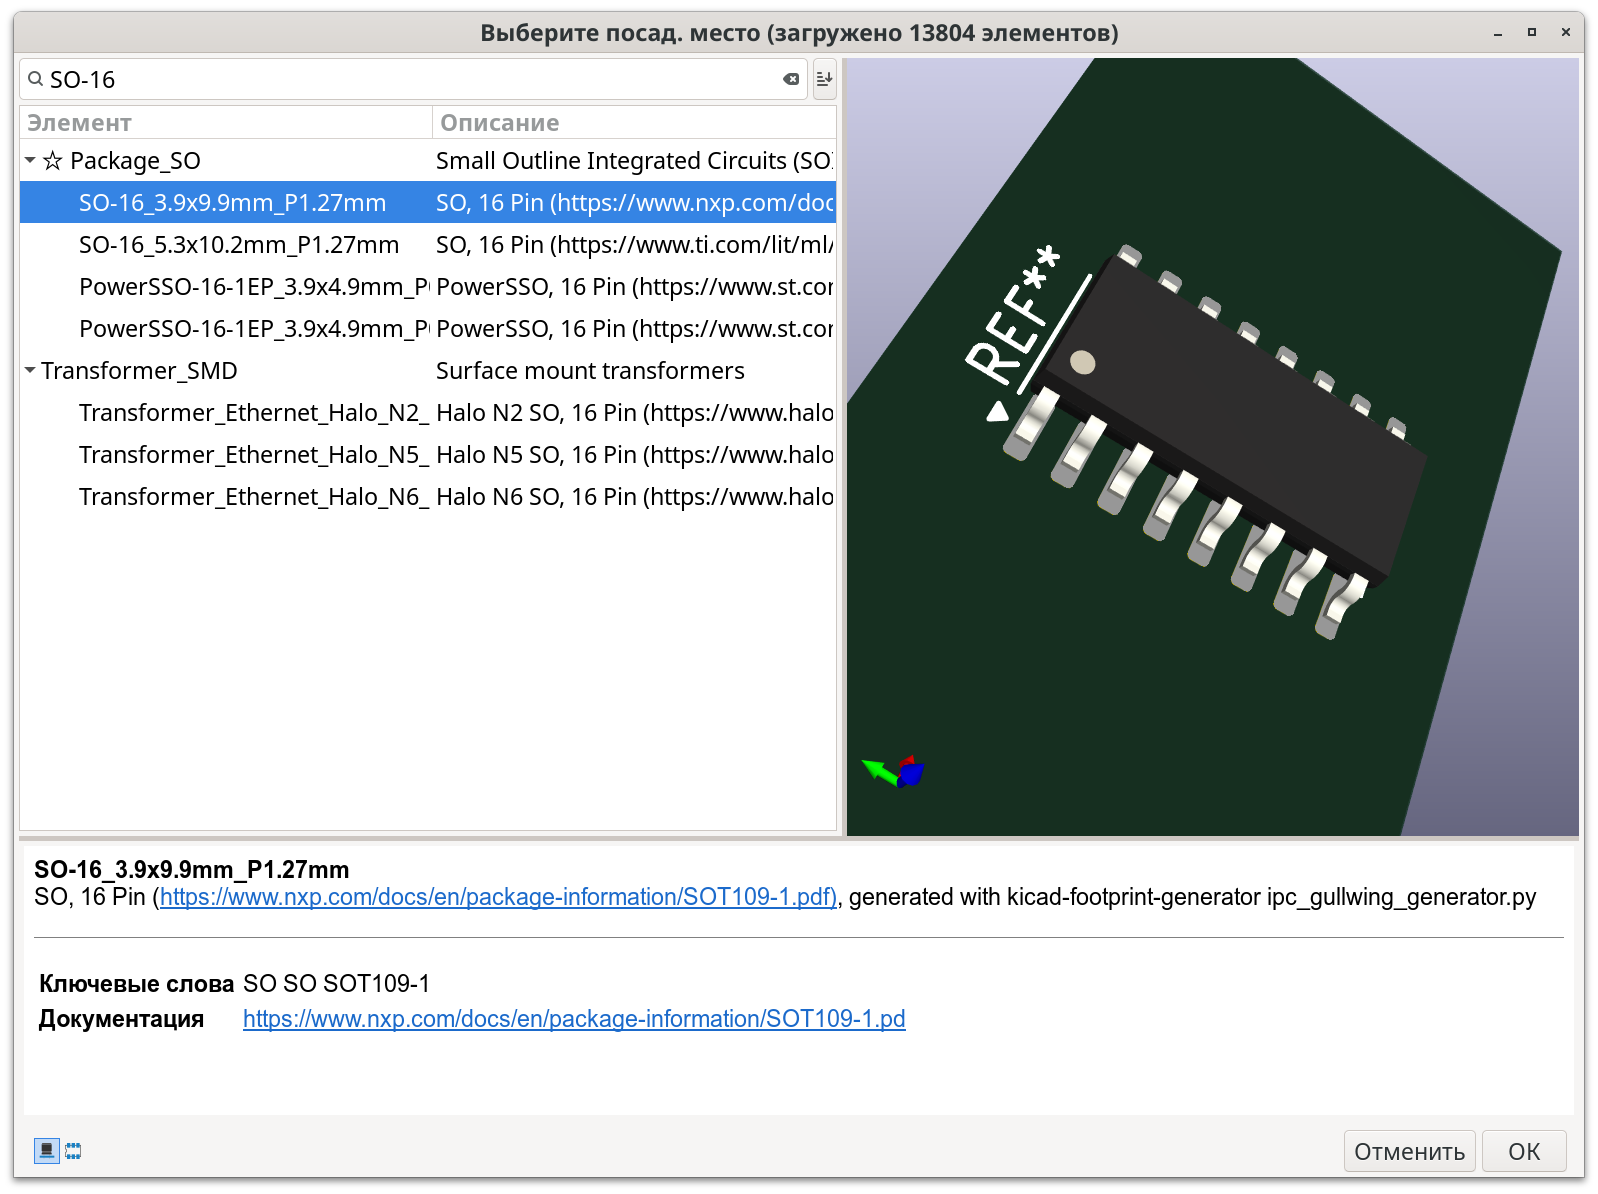
\includegraphics[scale=0.2]{kicad-so-package-footprint-with-3d.png}
  \caption{Снимок экрана с меню выбора посадочных мест в \textit{kicad-pcbdoc}}
\end{figure}

Точно также мною была найдена готовая
схемная библиотека соответствующая ГОСТ. 
% https://github.com/KiCad-RU/kicad-symbols-gost

% Скриншот окна со схемной библиотекой по ГОСТ
\begin{figure}[H]
  \centering
  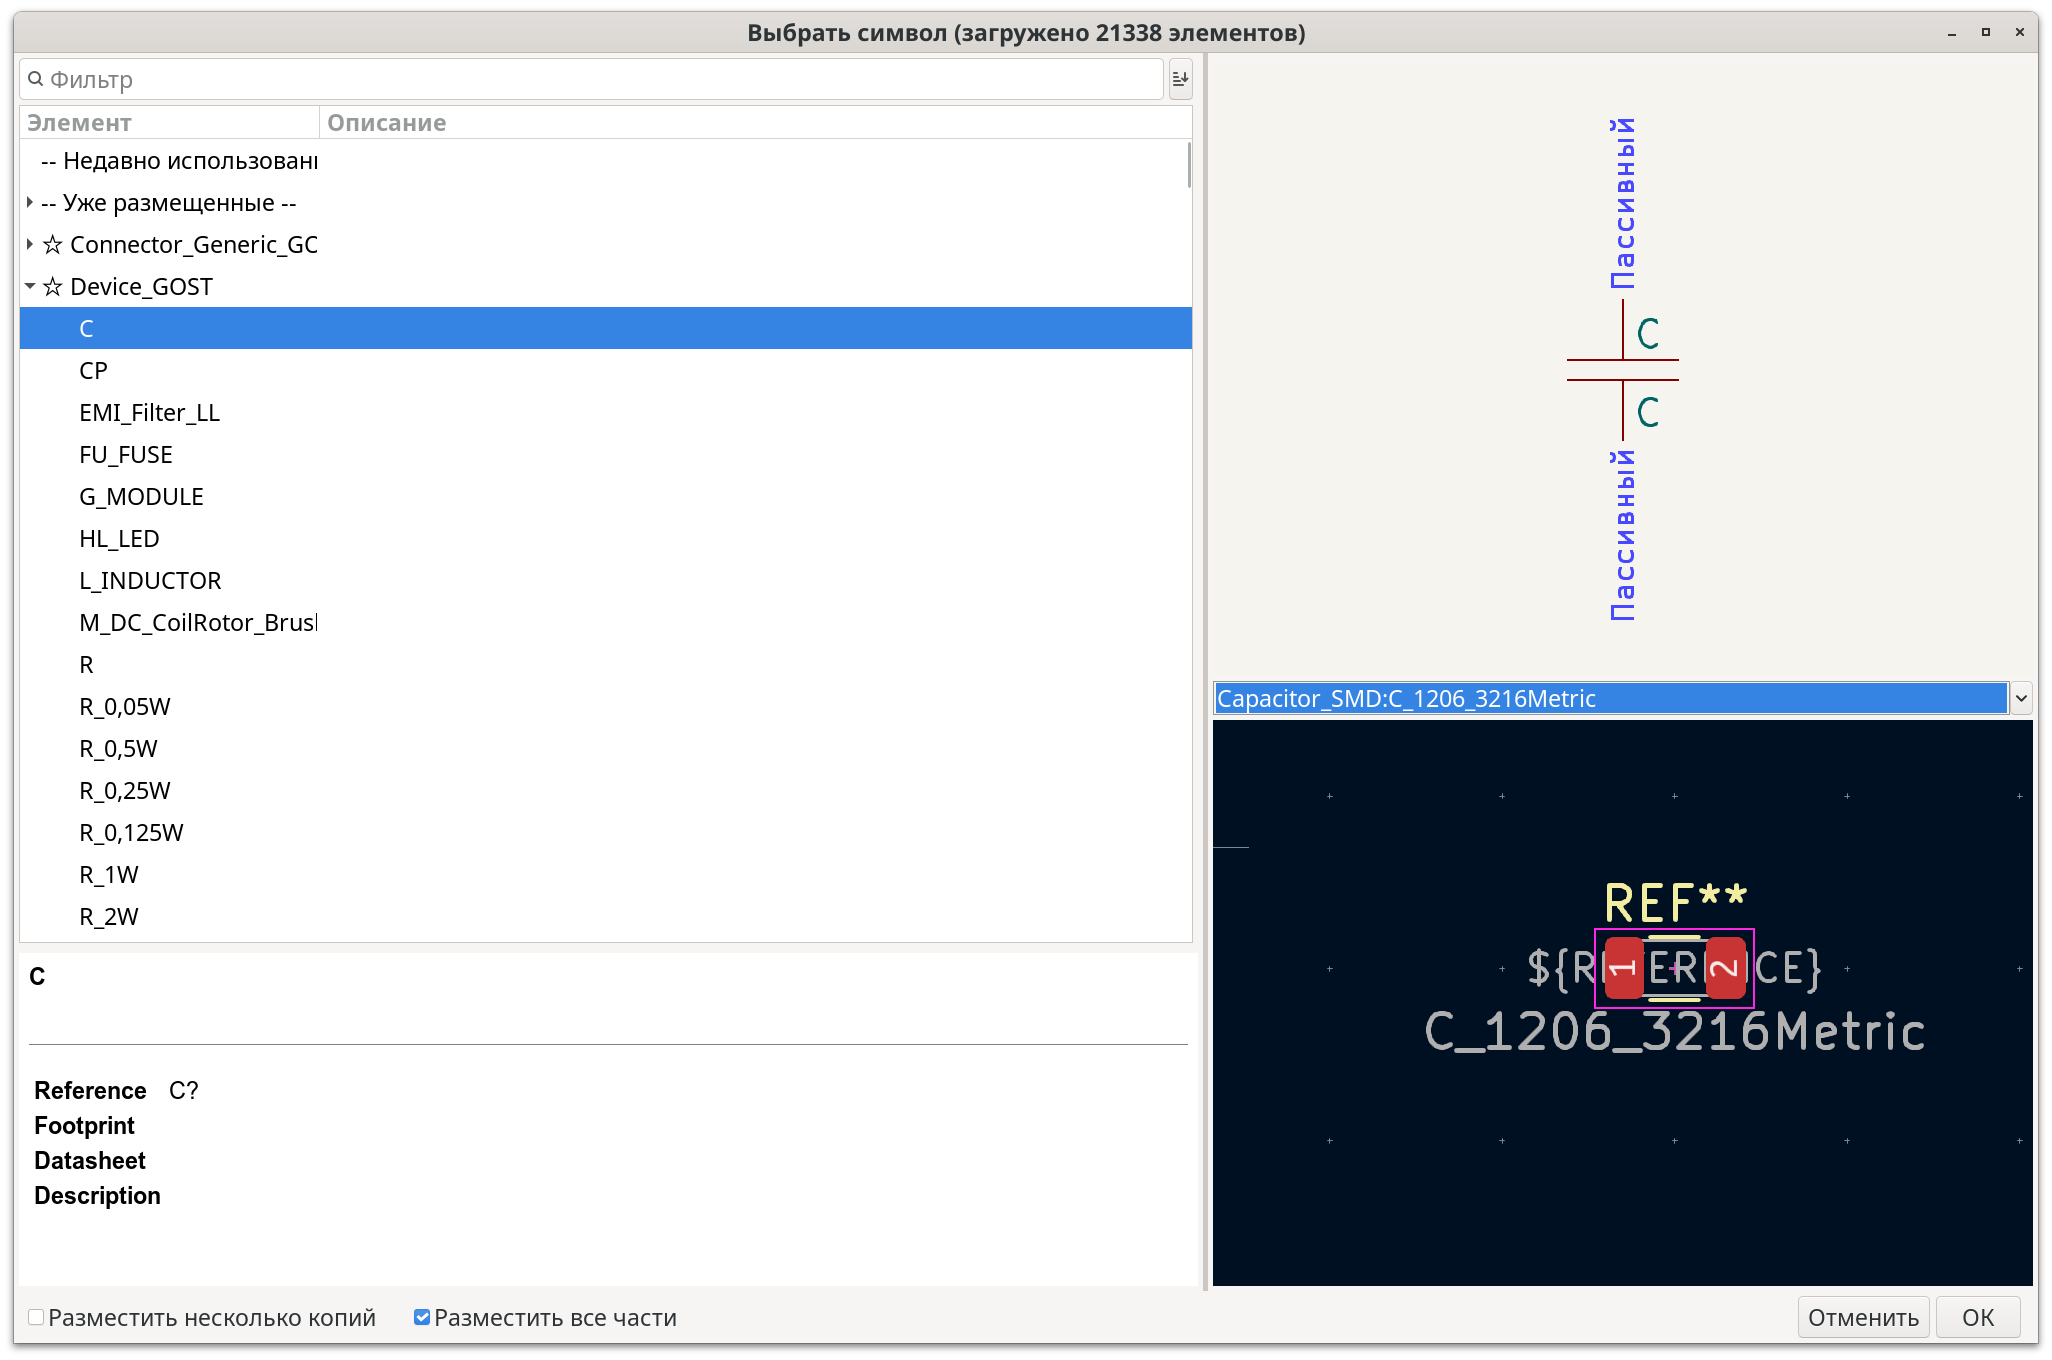
\includegraphics[scale=0.2]{kicad-capacitor-gost-library.png}
  \caption{Снимок экрана с меню выбора cхемных компонентов
    мест в \textit{kicad-eeschema}}
\end{figure}


Упорно работая я пришел к результату,
когда верификация принципиальной схемы «\textit{ERC}»
не показывала предупреждений о нарушении.

Спустя несколько дней к такому же результату,
я пришел выполняя верификацию разведённой печатной платы «\textit{DRC}».

Однако прохождение верификации не уберегло,
меня от схемотехнической ошибки,
с неправильно подключенным транзистором.
Тут могло помочь только внимание к сложным местам,
потому что именно место, где я далее допустил ошибку,
изначально показалось мне самым сложным, как в создании схемы,
так и в трассировке платы.

\newpage

% Local Variables:
% compile-command: "sh build.sh"
% End:
